%=========================================================================
% (c) Michal Bidlo, Bohuslav Křena, 2008

% Start of text
\chapter{Introduction}

Focus of this thesis is a performance optimization of BeakerLib library, particularly its Journal feature. 

\chapter{Relevant projects}

In this chapter describes BeakerLib and projects relevant to it.

\section{BeakerLib}

BeakerLib is a shell-level integration testing library, providing convenience functions which simplify writing, running and analysis of integration and blackbox tests. 
It is developed and maintained by Red Hat and operates under GNU General Public License.
Main features of BeakerLib include:
\begin{itemize}
\item Journal - uniform logging mechanism. 
\item Phases - logical grouping of test actions, clear separation of setup / test / cleanup
\item Asserts - common checks affecting the overall results of the individual phases (checking for exit codes, file existence and content...)
\item Helpers - convenience functions for common operations such as managing services, backup and restore 
\end{itemize}
[citace beakerlib github wiki]

This thesis focuses on BeakerLib Journal and problem it causes with long tests.


\section{Beaker}

Beaker is a full stack software and hardware integration testing system, with the ability to manage a globally distributed network of test labs.  [citace beaker doc] It is Red Hat community project under GNU General Public License version 2.

Main functionality includes management of hardware inventory, on which Beaker can install wide variety  of operating systems from Red Hat Linux family. Another notable part  is Task library which contains rpm packages of individual tests which can be run on provided machines. 
Users then can with specify which hardware they require with which OS and tests they want to run on it through either command-line tools or web interface both of which are part of Beaker install package [link to beaker download page ??? ]. If Beaker meets given criteria in its inventory it installs Test harness to which it gives list of tests to be run.  After Test Harness finishes running the tests, results are sent back to Beaker where they are stored for specified period of time. 

\subsection{beaker-wizard}
Part of Beaker package. Interactive command-line tool which automates creation of BeakerLib tests. Using predefined or user-defined templates it creates all files that are needed to run BeakerLib test.

\section{Test Harness}
Test harness is a software framework that automates test execution. It contains tests to be run, executes them and reports results. <expand>

Beaker’s harnesses prepare provided machine for BeakerLib by setting environmental variables to proper values, and then running the tests.

\subsection{Beah harness}
Beah [link to doc] is a default Beaker harness . <expand> 

\subsection{Restraint harness}
Restraint [link to doc] is an alternative Beaker harness which can, unlike Beah, run with Beaker or standalone without it. <expand>
\\
\\
Relations between Beaker, Harness and BeakerLib is shown in figure \ref{fig:beaker_relation}

\begin{figure}[h!]
  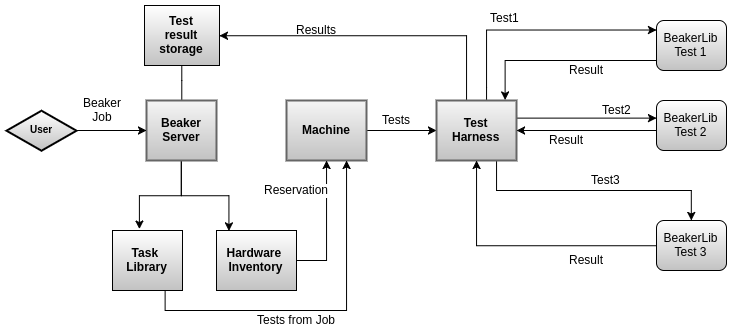
\includegraphics[width=\linewidth]{beaker_relations.png}
  \caption{Beaker relation to BeakerLib}
  \label{fig:beaker_relation}
\end{figure}




\chapter{BeakerLib}
This chapter explains inner workings of BeakerLib more in-depth, with focus on Journal feature, its problems and proposed optimizations.
\\
\\
As stated earlier BeakerLib is shell-level library with functions that make writing and running tests easier as well as examining their results.
BeakerLib adds testing functions to \textit{shell} functionality, so user can combine normal \textit{shell} commands and constructions with helping functions which can make writing tests and examining their results easier. There is around 80 of these functions, descriptions of most used ones follows:
\begin{itemize}
\item \textbf{rlRun} - First argument of this function is any shell command, which is executed by rlRun. Second is an expected exit code of first argument, it can contain one or more codes. Third argument is a comment. BeakerLib logs FAIL or PASS if expected exit code differs or not from actual one respectively along with comment. This is most used and important function.
\item \textbf{rlPass} - Manual assertion and logging of PASS. Useful when in combination with if statement which user doesn't want to appear in logs but still wants to log its result. Reciprocal function \textbf{rlFail} exists as well.
\item \textbf{rlAssertExists} - Asserts whether file given as a first argument exists.
\item \textbf{rlAssertGrep} - Function logs PASS when pattern given as first argument matches in a file which a second argument. Optional flags are passed to \textit{grep} and behave the same way.
\item \textbf{rlAssertRpm} - Function asserts PASS when package given as first argument is installed.  Optional arguments allow specifying particular version, release or arch of the package.
\item \textbf{rlAssertDiffer} - Asserts whether two files given as argument differ in their content. 
\end{itemize}
~\\
BeakerLib divides tests into logical groups called Phases. There are three basic types of phases:
\begin{itemize}
\item Setup - preparing conditions for the test (such as creating temporary files, starting needed services and so on)
\item Test - main phase for testing
\item Cleanup - reverting changes made by the test
\end{itemize}
This division helps when examining the result of test as it shows which phase causes fail, if any, in BeakerLib's output. Example test \ref{lst:test_example} shows how basic BeakerLib test looks.
\\
\begin{lstlisting}[style=beakerlib_bash,caption={BeakerLib basic test example},label={lst:test_example}]
# Include Beaker environment
. /usr/bin/rhts-environment.sh || exit 1
. /usr/share/beakerlib/beakerlib.sh || exit 1
# Start of Journal
rlJournalStart
    # Start of Setup Phase, creating temp directory where test will take place 
    rlPhaseStartSetup
        rlAssertRpm $PACKAGE
        rlRun "TmpDir=\$(mktemp -d)" 0 "Creating tmp directory"
        rlRun "pushd $TmpDir"
    rlPhaseEnd
   # Start of Test Phase, testing touch and ls commands
    rlPhaseStartTest
        rlRun "touch foo" 0 "Creating the foo test file"
        rlAssertExists "foo"
        rlRun "ls -l foo" 0 "Listing the foo test file"
    rlPhaseEnd
   # Statr of Cleanup phase, temp directory is deleted
    rlPhaseStartCleanup
        rlRun "popd"
        rlRun "rm -r $TmpDir" 0 "Removing tmp directory"
    rlPhaseEnd
rlJournalPrint
rlJournalEnd
\end{lstlisting}


\section{BeakerLib's output}
BeakerLib produces 3 kinds of outputs 2 files and terminal one. Files are saved into directory created for each individual test. If the test is run locally temporary directory is created on system with \textit{mktepm} command. If run on Beaker unique \textbf{TESTID} is generated for each test. This TESTID serves as a name for test directory as well as identifier which Beaker later uses when connecting test results with correct test.

\subsection{journal.txt}
\textit{journal.txt} is a plain text file with human readable record of test's progress. After end of each phase, copy of the file is sent to Beaker for storage.
\subsection{Terminal output}
If the executed test is connected to an \textit{interactive shell} the same BeakerLib's output is printed to terminal's standard output (\textit{stdout}) as well as to journal.txt. However \textit{shell's} output is colored for increased readability.  

\subsection{journal.xml}
Last output is XML[abbre???] file. This file is stripped off of commands' output, but core information (such as which commands were executed, whether they passed or failed and so on) is kept. Also metadata about the test run (time of execution, which component was tested and more) as well as information about the hardware and software test was run on are added. \textit{journal.xml} is sent back to Beaker same as \textit{journal.txt} where it is available for further processing.

\section{Journal problem}

\section{Proposed solutions}

\subsection{Change of xml parser}

\subsection{Change in accessing journalling.py}

\subsection{Queue file solution}

\subsubsection{(Dis)advantages}

\subsubsection{Queue file}

\subsubsection{Escaping}


\subsection{Daemon-like solution}

\subsubsection{(Dis)advantages}

\subsubsection{Signals}

\subsubsection{Escaping}



\chapter{Performance measuring}
<Definition of performance measuring>

For performance measuring of BeakerLib I chose two kinds of tests in in two kinds of testing environments.

\section{Tests}

\subsection{Artificial tests}
First type of tests are artificial tests created by me with beaker-wizard* to specifically target and measure performance of journalling modification I made. They consist mostly of commands that directly work with journalling.xml. For example commands rlLog or rlPhaseStart and rlPhaseEnd. That way we can observe clear difference in performance without being affected by operations unrelated to journalling (executing actions that verify functionality of components in real tests). 

<description of artificial tests with links to Appendix>

\subsection{Real tests}
Second type are real tests used in Red Hat. These are examples of tests that have been reported to have bad performance with BeakerLib so I am testing them to see if my modifications have real life impact on performance.

<description of real tests>

\section{Testing Environment}

\subsection{Local}
First environment is local laptop for convenience and speed of execution. I measured  two parameters, time of execution of each test and memory usage during execution. Tests were run directly, without any harness and with these technical specifications. 

<table of tech specs>

\subsection{Remote in beaker}
Second round of testing was done to emulate real testing conditions and to verify that changes made to BeakerLib do not break functionality outside of controlled environment. Tests were run with the default test harness Beah. Only overall time of execution of each test was measured in remote testing.

<table of tech specs>

\section{Baseline measurements}
<results>


\section{Implemented optimizations}
<results>

\chapter{Conclusion}
Recap of results
\\
Future work


%=========================================================================
